\section{Анализ предметной области}

\subsection{Задача обнаружения и прогнозирования ошибок и сбоев на станке лазерной резки Навигатор}

Основным объектом исследования данной работы является станок лазерной резки Навигатор
компании ВНИТЭП. Данный станок установлен в компании Сеспель,
занимающейся производством автоцистерн и полуприцепов для различных видов перевозок:
бензовозы, зерновозы, самосвальные прицепы, цементовозы и т.д.

Опишем функциональный и модульный состав данного станка, а также обозначим
проблему обнаружения и прогнозирования ошибок и сбоев для станка.
Кроме этого, опишем подход для решения данной задачи через автоматизацию.

\subsubsection{Описание комплекса Навигатор КС-12В}

\begin{figure}[h]
    \center{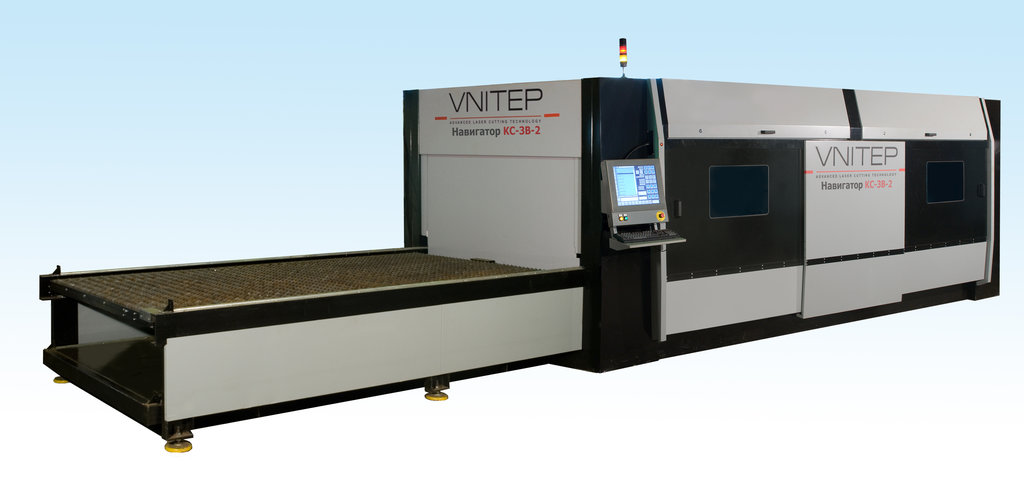
\includegraphics[width=10cm]{navigator.jpeg}}
    \caption{Внешний вид комплекса Навигатор КС-12В}
    \label{navigator}
\end{figure}

Навигатор КС-12В (рисунок \ref{navigator})  представляет собой комплекс обработки листового металла с волоконным лазером,
линейным синхронным двигателем и числовым программным управлением (ЧПУ).
Разработкой и поддержкой данного комплекса занимается Российская компания ВНИТЭП.
Станок является основным продуктом данной компании.

\begin{figure}[h]
    \center{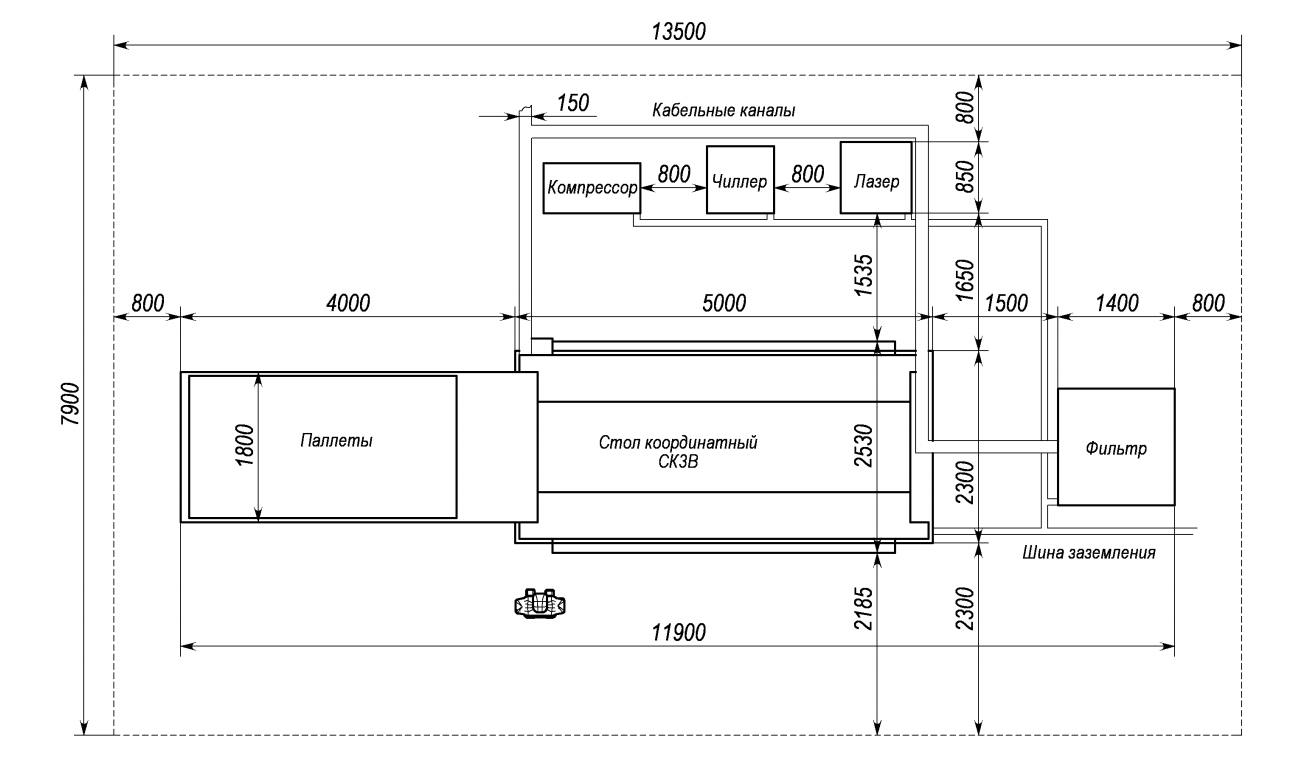
\includegraphics[width=14cm]{navigator.png}}
    \caption{Графическое описание основных частей станка}
    \label{modules}
\end{figure}

Комплекс состоит из следующих основные модулей (рисунок \ref{modules}):
координатный стол, иттербиевый лазер, компрессор, установку для фильтрации и вентиляции, чиллер.
Координатный стол состоит из пульта ЧПУ с программным обеспечением,
линейных моторов, линейных шариковых направляющих,
кабельных каналов, предохранительных каналов,
паллет для сбора технологических отходов,
оптической измерительной системы.

Возможности станка покрывают задачи лазерной резки большинства металлов различной толщины, до 30 мм.
Основные используемые металлы: бронированная сталь, нержавеющая сталь, цирконий, латунь.

Для работы со станком оператор загружает программу через интерфейс ЧПУ.
Загружаемая программа представляет собой набор инструкций для станка,
которые выполняет станок для вырезки определенной детали определенного формата.

Объектом дипломной работы является модель описанного станка.
В компании Сеспель используются несколько станков данной модели.

Задача дипломной работы будет решаться в контексте
системы компании Omnicube.

Компания Omnicube разрабатывает и предоставляет универсальную платформу
для решения разнообразных задач интеллектуального мониторинга
на предприятиях различных отраслей: промышленность,
интеллектуальные сервисы для зданий, мониторинг персонала,
экологический мониторинг, сервисы для предприятий сельского хозяйства,
инструменты для медицинских учреждений. \cite{omnicube}

Одним из клиентов компании Omnicube является предприятие Сеспель.
Компания Omnicube предоставляет функционал сбора, обработки и отображения
данных устройств предприятия: станки, установки, производственные роботы. 
Сами данные собираются с интегрированных и установленных датчиков этих устройств.
Кроме этого, Omnicube предоставляет
пользовательский интерфейс для руководства и сотрудников компании Сеспель.
На данном интерфейсе отображена статистика по различным параметрам,
а также отображены различные статистические показатели.

\begin{figure}[ht!]
    \center{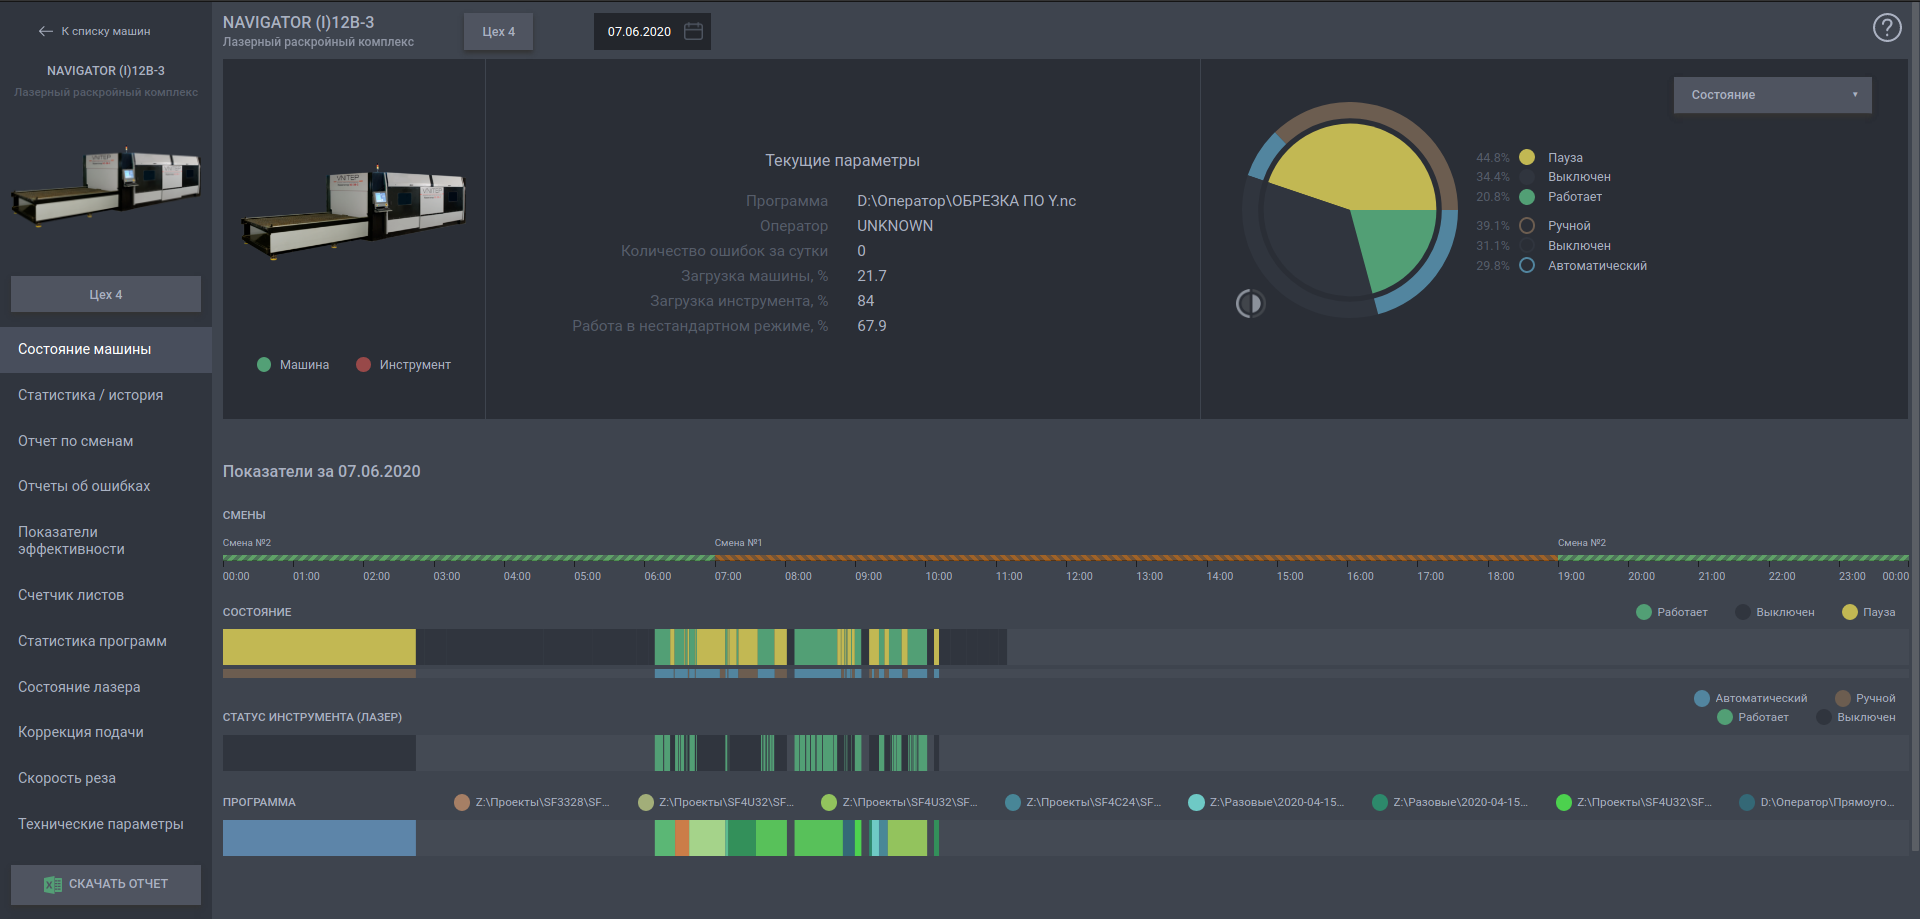
\includegraphics[width=16cm]{general.png}}
    \caption{Главные показатели работы станка}
    \label{main}
\end{figure}

Главными показателями (рисунок \ref{main}), которые отображаются в интерфейсе являются:
состояние, статус лазера, работающая программа.
Все показатели записываются относительно рабочий смен сотрудников.
Параметр состояния отображает текущий режим работы станка
и представляет собой три режима: рабочий (работа),
выключенный (выключен), пауза.
Показатель статус инструмента (лазера) отображает
статистику по работе лазера станка и может иметь режимы:
автоматический, ручной, рабочий, выключенный.
Рабочий режим представляет собой использование лазера под присмотром оператора.
Кроме этого, основным показателем также является статистика используемых программ для станка.

Вся статистика ведется ежедневно, так как работа ведется посменно.
Данную статистику можно проверить в разделе статистика-история.
Кроме этого, собирается статистика в виде отчета по сменном каждого оператора.


\begin{figure}[ht!]
    \center{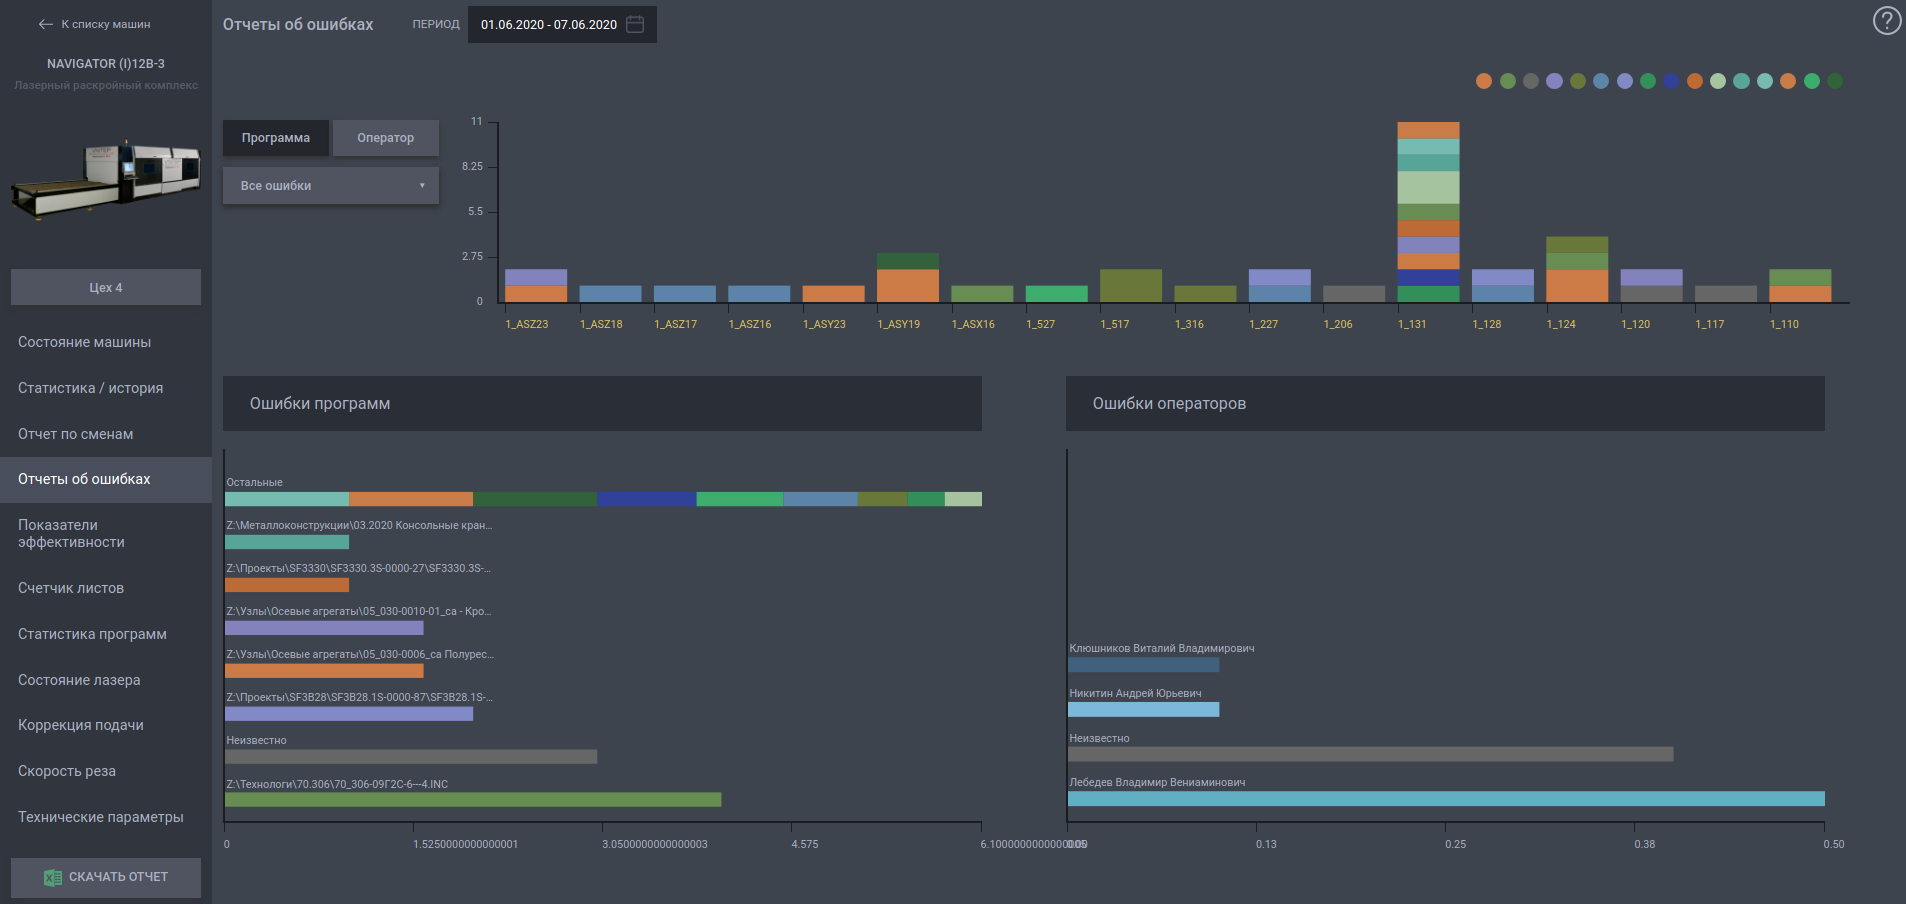
\includegraphics[width=16cm]{errors.png}}
    \caption{Отчет об ошибках программ и операторов}
    \label{errors}
\end{figure}



\begin{figure}[ht!]
    \center{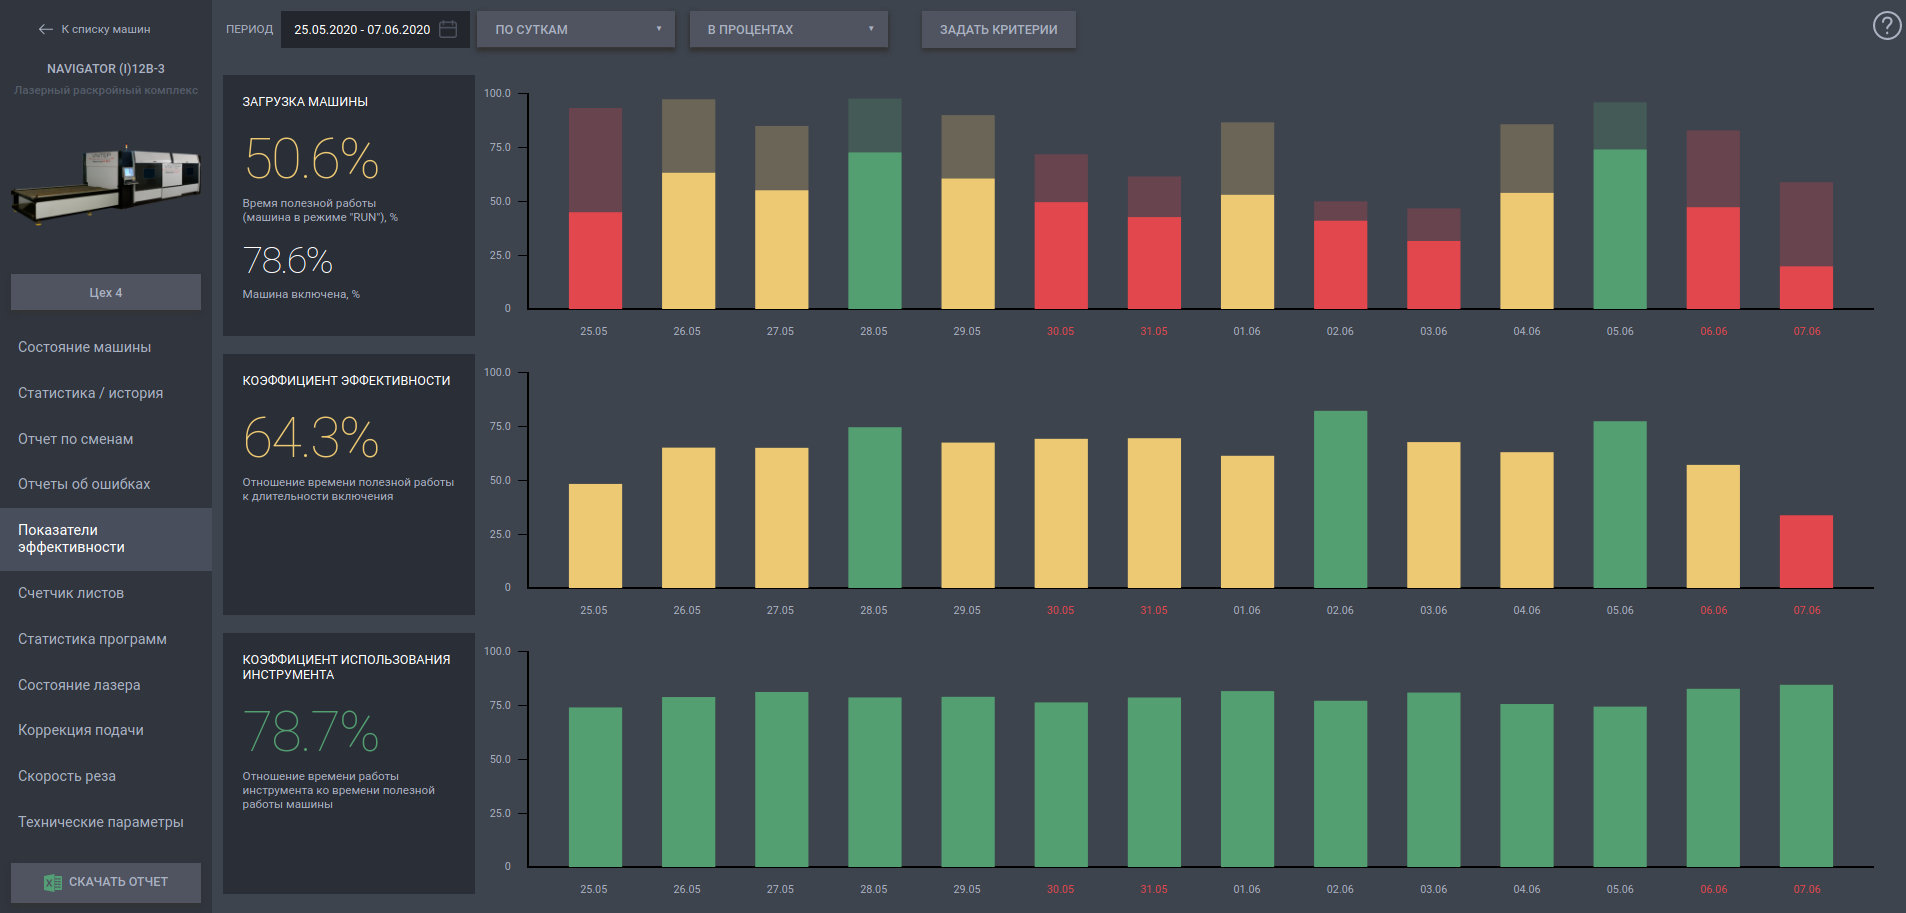
\includegraphics[width=16cm]{effective.png}}
    \caption{Показатели эффективности}
    \label{effective}
\end{figure}

В разделе <<Отчеты об ошибках>> (рисунок \ref{errors}) отображается статистика
по неисправностям работающих программ и по ошибкам операторов.
В основном графике можно увидеть количество возникновения
ошибки (по оси Y), имеющей определенный код (ось X)

Раздел <<Показатели эффективности>> (рисунок \ref{effective}) содержит показатели
загрузки машины, коэффициента эффективности
и коэффициента использования инструмента.
Параметр <<Загрузка машины>> представляет собой
время полезной работы.
<<Коэффициент эффективности>> -- отношение времени полезной работы
к длительности включения.
<<Коэффициент использования инструмента>> -- отношение времени работы
инструмента ко времени полезной работы машины.
Все показатели выражены в процентах, либо в часах.
Также возможно проверить показатели как по сменам,
так и по часам.

\begin{figure}[ht!]
    \center{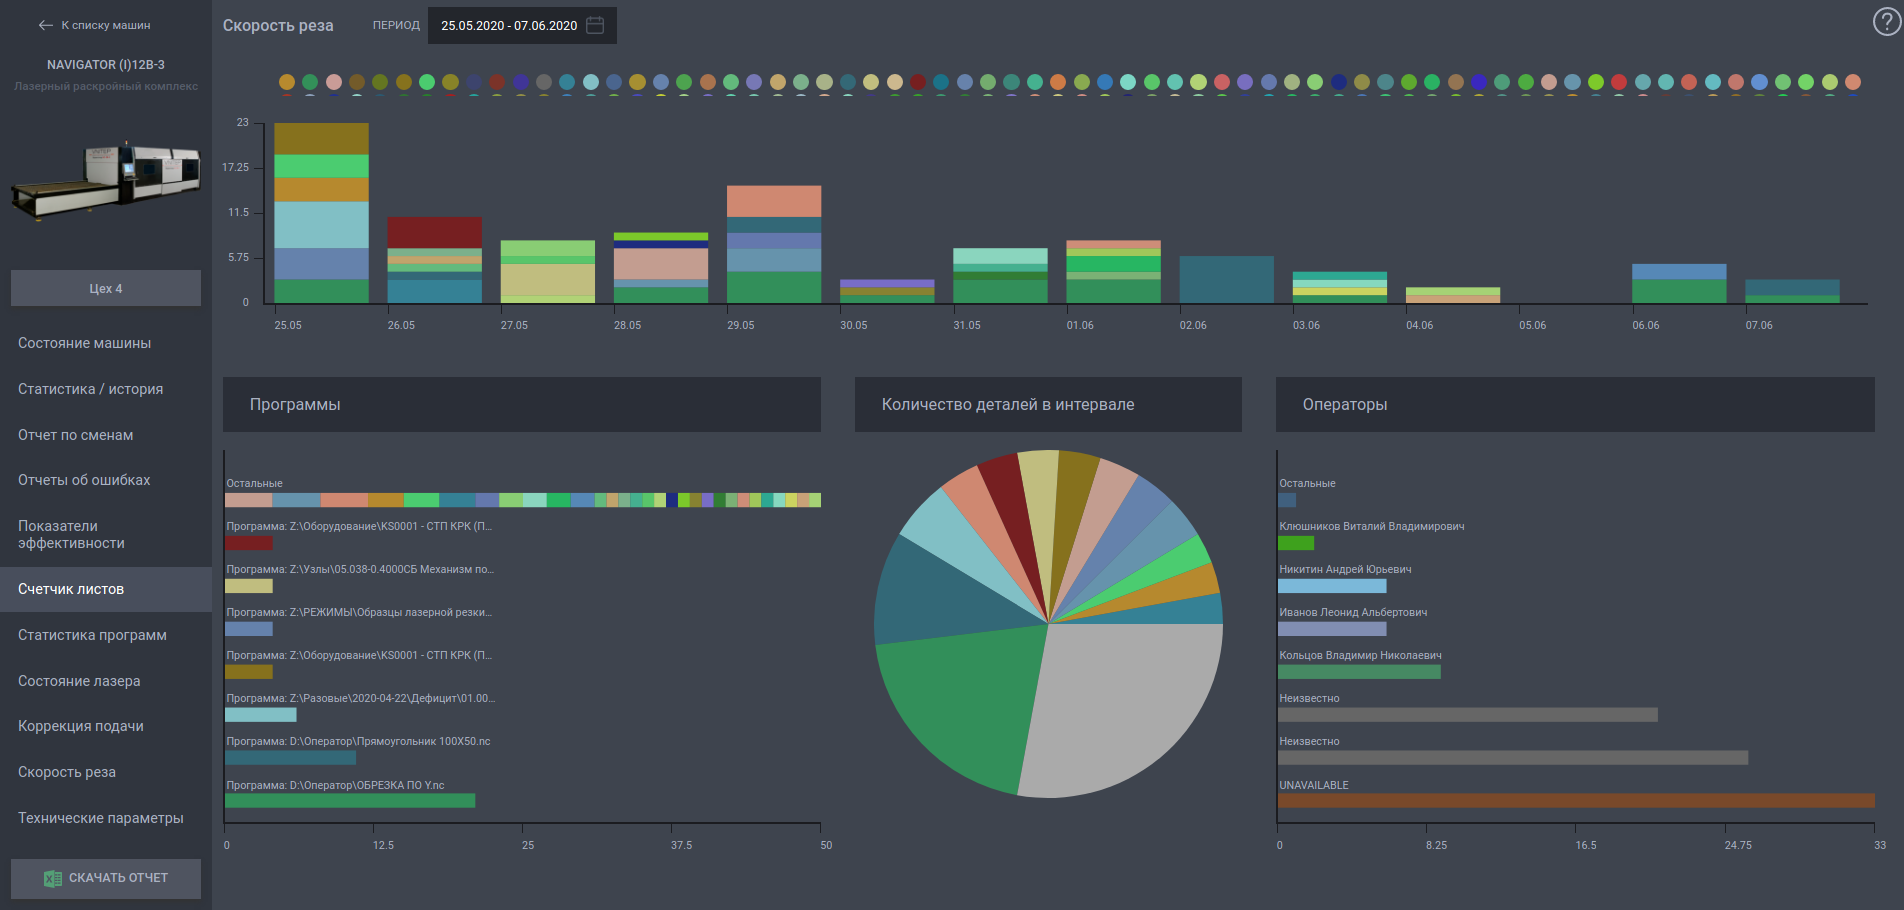
\includegraphics[width=16cm]{counter.png}}
    \caption{Статистика счетчика листов}
    \label{counter}
\end{figure}

Раздел <<Счетчик листов>> (рисунок \ref{counter}) отображает статистику по количеству
загружаемых в станок металлических листов.
Для просмотра статистики можно выбрать желаемый период.

\begin{figure}[h]
    \center{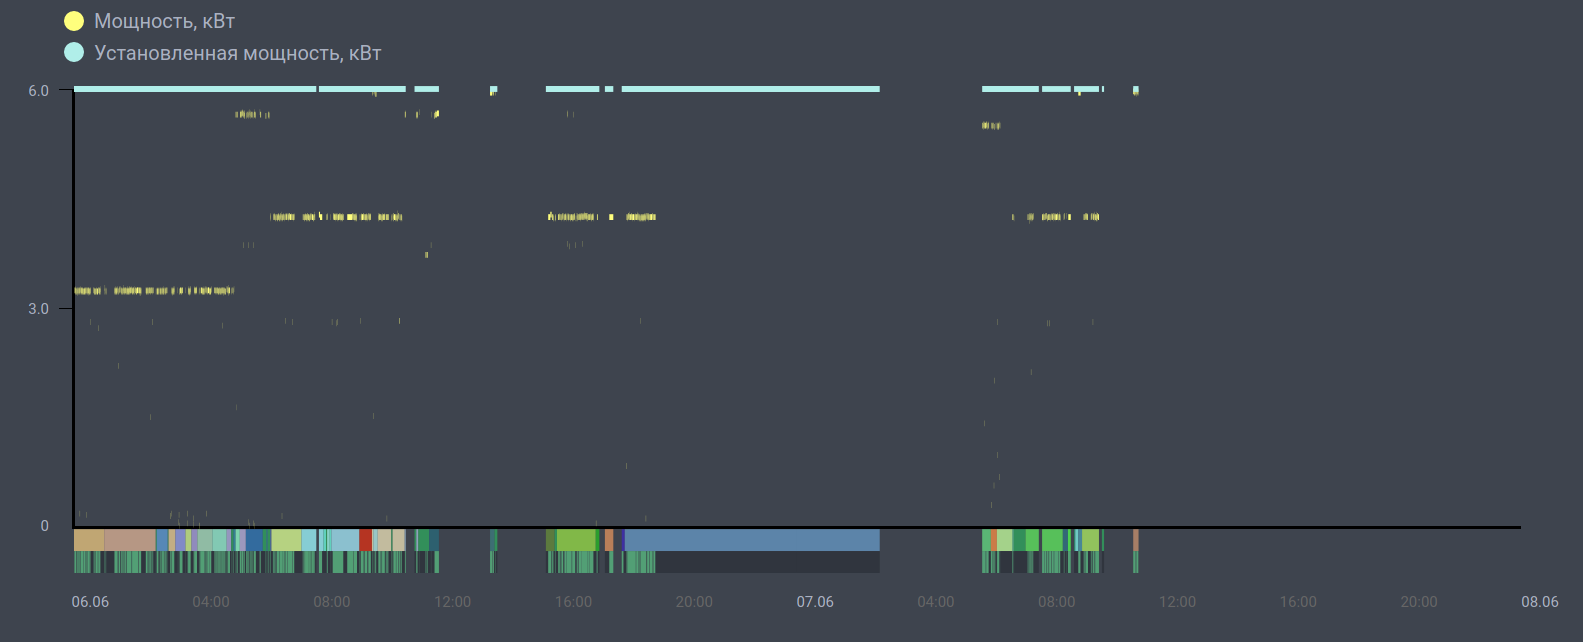
\includegraphics[width=16cm]{laser_power.png}}
    \caption{Статистика по используемой мощности лазера}
    \label{laser_power}
\end{figure}

\begin{figure}[h]
    \center{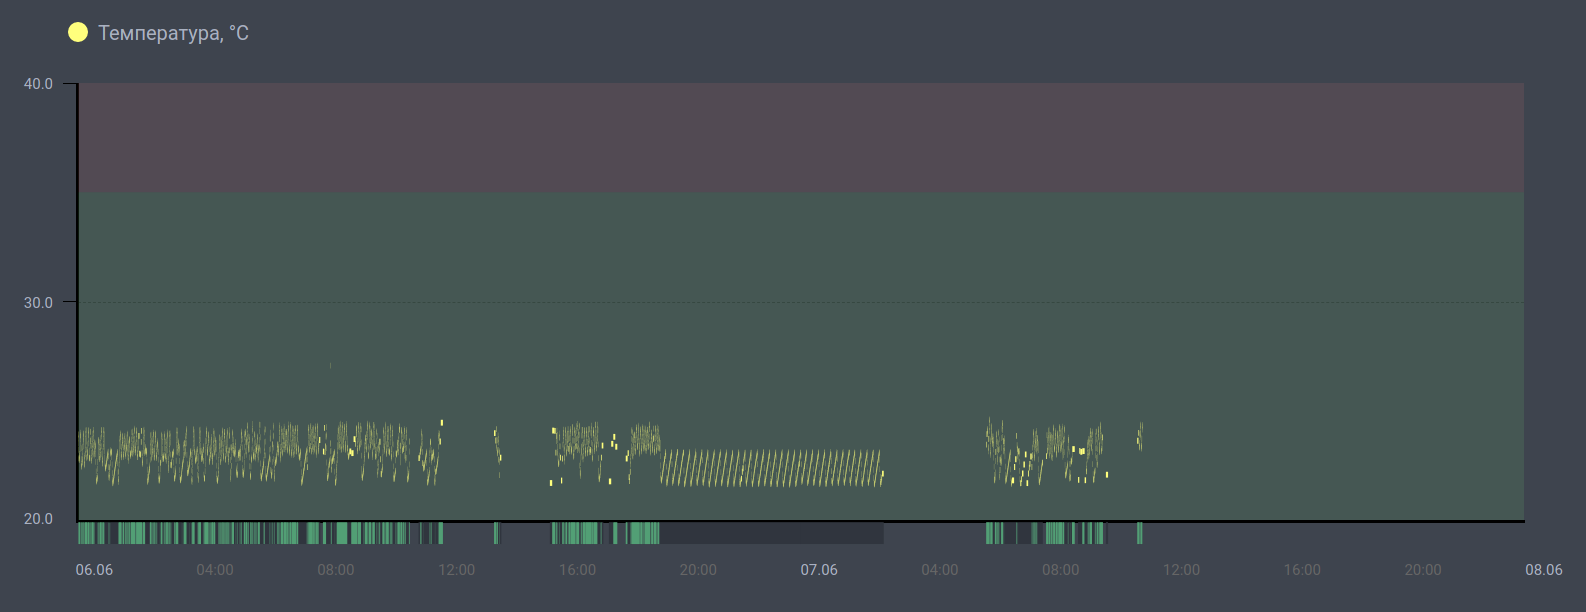
\includegraphics[width=16cm]{laser_temp.png}}
    \caption{Статистика по температуре источника}
    \label{laser_temp}
\end{figure}

Раздел <<Состояние лазера>> содержит три показателя по
состоянию лазера в течение использования:
отношение фактической мощности лазера к заданной,
мощность фактическая и установленная (рисунок \ref{laser_power}), температура источника лазера (рисунок \ref{laser_temp}).

Кроме этого есть еще разделы:
<<Статистика программ>> -- статистика по используемым программам;
<<Коррекция подачи>> -- отклонение по программам и операторам;
<<Скорость реза>> содержит данные по скорости реза,
коррекции скорости реза, а также данную статистику относительно программ и операторов.
Также можно ознакомиться с основными техническими характеристиками данного станка,
а также загрузить отчет в формате .xls, в котором будет содержаться вся статистика
по всем показателям за обозначенный промежуток.

\subsubsection{Проблема диагностики неисправностей}

Эффективная эксплуатация промышленных устройств
требует наличия надежных обслуживающих систем,
которые должны предоставлять безопасные, отказоустойчивые решения,
поэтому предотвращение ошибок и сбоев имеет первостепенное значение.

Обычно, чтобы предотвратить сбои и ошибки, операторы,
как правило, выполняют техническое обслуживание 
на основе рекомендаций производителей, 
и им приходится регулярно проверять критически важные детали,
Для этого требуются опытные специалисты с высоким уровнем квалификации.
Данный процесс очень дорог и трудоемок.

Данная проблема присутствует и на станках модели Навигатор.
Регулярно возникают ситуации ошибок программного обеспечения
и работы операторов, а также возможны критические сбои,
которые заключаются в отказе оптической системы (лазера).
Также возможен износ оборудования,
например, сбой привода оси XYZ.

На данный момент операторам необходимо постоянно следить за состоянием
станка, проводить сложный технический анализ,
который может потребовать дополнительных специалистов.
Как уже говорилось, такой подход может занять много времени,
а также потребовать немало денежных ресурсов.
Такой подход является единственным для станков модели Навигатор.


\subsubsection{Автоматическое обнаружение неисправностей как решение проблемы диагностики неисправностей}

Целью данной дипломной работы является создание системы
для обнаружения и прогнозирования неисправностей на станках лазерной резки Навигатор.
Решение данной задачи представляет собой
разработку и внедрение данной системы,
а также описание теоретического обоснования.

Решение поставленной задачи принесет
положительные результаты как для компании ВНИТЭП,
так и для ее клиентов, в том числе для предприятия Сеспель,
а именно такое решение может сократить
время операторов и инженеров,
тем самым буду сэкономлены денежные и другие ресурсы
предприятия.
Разрабатываемое решение повысить эффективность
промышленных процессов предприятия Сеспель.

Основными средствами для решения поставленной задачи
будет собранная за период 2017-2019 статистика
по различным параметрам различных модулей:
ЧПУ, лазер, составные части.

Основными метриками будут:

\begin{itemize}
    \item Отношение заданной мощности лазера к фактической, которое позволит
    отслеживать тренд износа головы лазера;
    \item Температура лазера -- параметр, который может также быть признаком износа
    лазерной головы, а также может быть предупреждающим параметром о возможном отклонении
    от нормы необходимой температуры, что может классифицироваться как ошибка оператора или ошибка станка в целом;
    \item Данные с датчиков вибрации -- позволяют отследить тренд изнашивания платформы станка;
    \item Данные с датчиков привода XYZ -- позволяют определить ошибки и сбои пространственного приводы лазера.
\end{itemize}




\subsubsection{Описание подхода к решению задачи автоматической диагностики}

В последнее время получила свое распространение
парадигма промышленного интернета вещей,
являющаяся частью более общего понятия -- интернета вещей,
которая предоставляет идеи объединения
промышленного оборудования и датчиков в единую систему.
Такая система может позволить проводить автоматизированный мониторинг и 
анализ критически важных параметров промышленных устройств,
без участия операторов, для обнаружения и предсказания ошибок и сбоев \cite{iiot}.

Не смотря на то, что парадигма промышленного интернета вещей предоставляет идеи
для создания системы, она не дает описания способов и методов реализации этой системы.
Такое положение обусловлено относительно недавним появлением данной парадигмы,
из-за чего еще не устоялась методология и принципы разработки.

Так как на данный момент нет устоявшихся концепций,
ведутся разработки на основе различных подходов,
при этом учитывается специфика промышленных устройств,
для которых разрабатывается система.

Проблему разработки системы промышленного интернета вещей можно разбить на две подпроблемы,
каждую из которых можно решать отдельно, однако решение второй подпроблемы может зависить от решения первой:

\begin{enumerate}
    \item Разработка подсистемы сбора, обработки и хранения данных с различных устройств;
    \item Разработка подсистемы анализа данных для обнаружения и предсказания ошибок и сбоев.
\end{enumerate}

Решение первой подпроблемы может стать основной для решения второй подпроблемы,
так как для анализ данных требует наличие готовой среды, в которой
будет происходить анализ.

Если первая подпроблема может быть решена проектированием грамотной архитектуры и выбора подходящих инструментов,
то для решения второй задачи необходимо определиться с подходами и методами
получения прогнозов ошибок и сбоев, с учетом особенностей данных.

Можно сказать, что для того, чтобы иметь систему обнаружения и прогнозирования ошибок и сбоев устройств,
нужно решить две поставленные подпроблемы. Первая подпроблема не является темой данной дипломной работы
и выходит за ее рамки, однако, в работе будет описана с учетом преимуществ и недостатков существующая разработанная система,
в контексте которой будет решаться вторая подпроблема.

\subsubsection{Временные ряды}

Проблему предсказания и обнаружения ошибок и сбоев на станках можно охарактеризовать как задачу анализа временных рядов,
так как основные данные представляют собой последовательность событий,
разграниченных по времени.

Временные ряды -- серия точек данных, индексированных во временном порядке.
Анализ временных рядов представляет собой совокупность методов анализа данных временных рядов,
которые направлены на выявление значимых паттернов \cite{box-series} .

Временные ряды имеют темпоральную структуру, то есть упорядочены во времени,
тем самым анализ временных рядов отличается от перекрестных исследований,
в которых обычно используется анализ выборки или выборок из генеральной совокупности в определенный момент времени.
Кроме этого, анализ временных рядов отличается от пространственного анализа,
который имеет такую же фиксированную основу как и перекрестные исследования,
например, в пространственном анализе могут анализироваться географические объекты, без учета временной компоненты \cite{shumway-series} .

Существует классификация временных рядов  \cite{zhang-series} :

\begin{itemize}
    \item одномерные и многомерные;
    \item стационарные и нестационарные;
    \item линейные и нелинейные.
\end{itemize}

Пусть есть процесс $x_t$, где $t \geq 0$ или $-\infty < t < \infty $.

Одномерные представляют собой временной ряд, которые генерируется на основе одного атрибута,
а многомерный имеет больше одного, другими словами в одномерном случае $x_t$ представляет собой вектор,
а в многомерном $x_t$ определяется как матрица.

Данные временного ряда можно представить в виде $n\times d$ матрицы данных \cite{zaki}: 

\begin{equation} \label{data_matrix}
    \textbf{D} = 
    \begin{pmatrix}
    x_{1,1} & x_{1,2} & \cdots & x_{1,d} \\
    x_{2,1} & x_{2,2} & \cdots & x_{2,d} \\
    \vdots  & \vdots  & \ddots & \vdots  \\
    x_{n,1} & x_{n,2} & \cdots & x_{n,d} 
    \end{pmatrix}
\end{equation}

Вектор-строки вида:

\begin{equation}
    \textbf{x}_i = (x_{i,1}, ..., x_{i,d})
\end{equation}

\noindent в зависимсоти от предметной области имеют различные названия, например:
сущности, объекты, примеры и т.д.

Вектор-столбцы вида:

\begin{equation}
    \textbf{X}_j = (x_{1,j}, ..., x_{n,j})
\end{equation}

\noindent также могут иметь различные названия: атрибуты, свойства, переменные и т.д.

Стационарность определяется через требование равносильности совместных распределений вектора
$(x_{t_1}, ..., x_{t_k})$ и вектора $(x_{t_1+t}, ..., x_{t_k+t})$.
Другими словами, в стационарном временном ряде есть повторяющиеся паттерны,
в отличие от нестационарного \cite{terence-series} .

Линейные модели определяются через свойства линейности параметров временного ряда, например среднего и дисперсии.
Нелинейные модели напротив могут иметь нелинейную структуру, что требует использования
нелинейных методов, например, методов нелинейной регрессии \cite{douglas-series} .

Самыми малоизученными являются нелинейные нестационарные модели \cite{rao-series} .
Примеры реализации системы обнаружения и предсказания ошибок,
основанные на данном типе моделей не были найдены и обсуждаться в данной работе не будут,
так как данная область выходит за рамки темы дипломной работы.

Обозначенную выше подзадачу можно разбить также на два элемента:

\begin{enumerate}
    \item выявление ошибок, обнаружение аномалий;
    \item п редсказание поведения устройства.
\end{enumerate}

Данные задачи можно решать как отдельно, где для каждой задачи будет использоваться свой метод,
так и совместно через один метод. Каждый вариант будет рассмотрен в существующих примерах.

\subsubsection{Интеллектуальный анализ данных временных рядов}

Также можно сказать, что поставленная задача обнаружения и предсказания ошибок и сбоев
является задачей интеллектуального анализа данных, а именно
интеллектуального анализа данных временных рядов.
Такое абстрагирование обосновано, так как существуют аналогичные задачи,
которые решаются именно с использованием данной парадигмы.

Интеллектуальный анализ данных (data mining) 
-- процесс выявления паттернов из больших объемов данных \cite{han-mining} .

\begin{figure}[h]
    \center{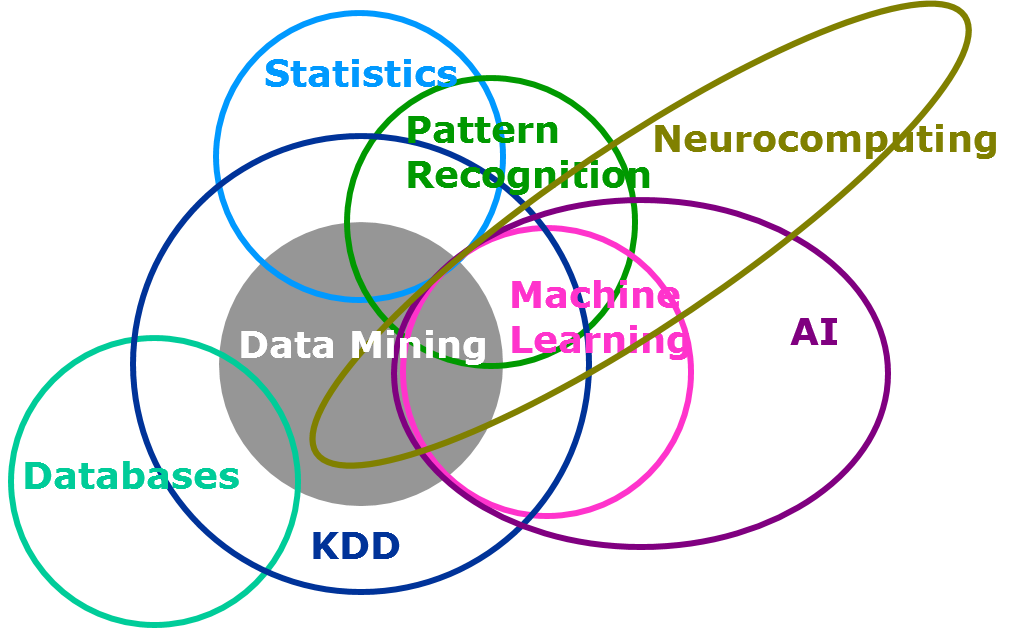
\includegraphics[width=10cm]{mining.png}}
    \caption{Место интеллектуального анализа данных среди других областей}
    \label{mining}
\end{figure}

Интеллектуальный анализ данных представляет собой междисциплинарную область,
в которой используются методы, идеи и принципы из следующих областей (рисунок \ref{mining}):
статистика, машинное обучение, распознавание образов,
вычислительная нейробиология, базы данных.
Стоит отметить, что данная область является частью более широкой области, 
которая называется выявление (обнаружение) знаний из баз данных (knowledge database discovery).

Кроме этого, интеллектуальный анализ данных можно определить как часть
распознавания образов/паттернов (pattern recognition),
которая связана с обработкой данных из баз данных и выявлением паттернов, 
связанных с определенной предметной областью \cite{mirkin-mining} .
Сама область распознавания образов покрывает и другие области, например,
обработка сигналов и машинное зрение \cite{mehmed-mining} .

Опишем приведенные области, обозначим их основные идеи и принципы.

База данных -- организованная коллекция данных, которая собирается и хранится
при помощи компьютерных систем.
Для взаимодействия пользователя с базой данных используется
система управления базами данных (СУБД).

Теория баз данных поставляет формализованные методы и принципы проектирования и разработки баз данных и СУБД.
Обычно теоретически выделяют два главных типа построения баз данных: реляционные (SQL) и нереляционные базы данных (NoSQL).
Также иногда выделяют смешанный тип, появившейся сравнительно недавно:
новые реляционные базы данных, который совмещает лучшие
идеи и принципы из реляционных и нереляционных теорий и подходов (NewSQL) \cite{fauler-db} .

В контексте интеллектуального анализа данных базы данных используются как источник данных.
Сами данные перед анализом обрабатываются, что также является частью процесса обнаружения знаний.
От типа и особенностей сбора и хранения данных в базе зависят последующие шаги анализа данных.

Обнаружение знаний из баз данных (knowledge database discovery, KDD) --  более широкая область
работы с данными из баз данных, частью которой является интеллектуальный анализ данных.
KDD определяют как процесс выявлений знаний (паттернов), который разбит на основные шаги  \cite{curr} :

\begin{enumerate}
    \item селекция -- выборка данных из баз данных по определенным критериям;
    \item обработка (pre-processing) -- приведение выбранных данных в подходящий вид 
    (очистка и удаление пропущенных значений, фиксирование атрибутов) для последующего анализа;
    \item трансформация (transformation) -- трансформация данных в подходящую структуру данных, например, в матрицу данных \eqref{data_matrix};
    \item интеллектуальный анализ данных (data mining) -- обнаружение паттернов в данных;
    \item интерпретация и оценка (interpretation and evaluation).
\end{enumerate}

Следующим шагом также может быть использование, развертывание и эксплуатация обнаруженных знаний и паттернов для целей предметной области.

Статистика, распознавание образов и машинное обучение являются поставщиками методов для каждого шага процесса KDD.
Каждая из этих областей имеет свои особенности, однако все они имеют также много общего.

\subsection{Анализ существующих решений задачи обнаружения и прогнозирования неисправностей в устройствах}

Итак, рассмотрим существующие решения для обнаружения аномалий, например, ошибок и сбоев в данных, а также
подходы к прогнозированию и оповещению об этом пользователей.

Во-первых, можно сказать, что модели прогнозирования временных рядов, такие как авторегрессивная модель (AR),
модель скользящего среднего (MA), экспоненциальная модель,
модель авторегрессии скользящего среднего (ARMA), 
интегрированная авторегрессионная модель скользящего среднего (ARIMA), 
зависят от параметров, полученных из исторических временных рядов. 
Эти параметры являются неотрицательными целыми числами, 
которые относятся к порядку авторегрессионной части, степени участвующей первой разности и порядку части скользящей средней. 
Хотя эти процессы могут обрабатывать нестационарные данные, 
они ограничены в запоминании любого состояния за любой промежуток времени \cite{nonlinear-series}. 

В \cite{3-paper} авторы рассмотрели потоковые данные как частично наблюдаемый Марковский процесс \cite{3-pomp}. 
Такое решение было принято с целью создания композиционной системы,
которая состояла из различных моделей: экспоненциальные модели, сезонные модели, модель лог-гауссовского процесса Кокса.
Данная статья содержит хорошие идеи использования фильтров на композиции частично наблюдаемых Марковских процессов, а также
теоретического обоснования такого использования. Однако, хорошая разработанная теория и слабое тестирование на реальных данных
не показало высокой эффективности такого подхода. В данной статье авторы научились только предсказывать аномалии,
но не смогли их определить, а также использовать данный подход в реальном времени.

Федеративное обучение -- один из это методов машинного обучения,
который состоит в обучении алгоритма на нескольких децентрализованных периферийных устройствах или серверах, 
содержащих локальные выборки данных, без обмена их выборками данных.
Использование федеративного обучения для фильтрации данных сети медицинских устройств было рассмотрено в \cite{8-paper}.
Благодаря использованию методов федеративного обучения, авторам удалось повысить энергоэффективность обработки и анализа данных,
то есть они решили одну из самых распространенных проблем в сфере интернета вещей.
Также в статье описаны этапы локального анализа данных на самих устройствах и глобального анализа данных на сервере.
Для первого этапа авторы использовали адаптивные фильтры \cite{adaptive-filter}, для второго матричный анализ возмущений \cite{pertuberation}.
Недостатком такого подхода является низкая гибкость, так как может потребоваться использовать корреляционный анализ устройств,
а в распределенном анализе корреляция может быть утрачена, тем самым будут утрачены полезные признаки.
Кроме этого, существуют усовершенствованные адаптивные фильтры, например ядерный рекурсивный фильтр \cite{krls-t}.
Еще можно сказать, что матричный анализ возмущений может не учитывать асинхронную структуру предобработанных данных.
 
В целях мониторинга профиля и обнаружения неисправностей в \cite{4-8} авторы применили модель нелинейной 
параметрической регрессии для разработки системы, которая была бы устойчивой и нечувствительной 
к изменениям температуры в производственной практике. 
В \cite{4-9} был разработан метод мониторинга, который может автоматически адаптировать параметры контрольной карты (метод из теории управления). 
В \cite{4-10} авторы добавили все профили каналов и применили анализ главных компонентов (PCA) 
агрегированным профилям тоннажа для извлечения характеристик. 
В \cite{4-12} использовались как статистические, 
так и вейвлет-характеристики, извлеченные из сигналов датчиков, 
для разработки адаптивного метода обучения для оценки износа инструмента в процессе высокоскоростного фрезерования. 
Каждое из этих исследований было сосредоточено на анализе индивидуального профиля данных, то есть анализ был проведен с одномерными данными.
Однако, выходы датчиков устройства обычно являются многоканальными, что требует многомерного анализа временных рядов.

У многомерных данных могут быть следующие особенности \cite{wei-series}: 
\begin{itemize}
    \item С увеличением числа датчиков обработка каждого 
    временного ряда от каждого датчика становится как более интенсивной, что сказывается на повышении вычислительной нагрузки;
    \item Данные имеют больше выбросов и шумов, по сравнению с одномерными данными;
    \item Временные ряды от разных датчиков имеют корреляции на разных уровнях, 
    что приводит к большому количеству избыточной информации, однако необходимо учитывать возможные корреляции;
    \item Состояния работы до простоя обычно продолжаются в течение некоторого времени и включают состояния отказа оборудования. 
    Кроме того, после восстановления неисправного датчика также появляется период задержки в рабочем состоянии. 
    Следовательно, модель прогнозирования должна иметь инвариантность памяти относительно таких состояний. 
\end{itemize}


Эти особенности данных приводят к следующим вопросам исследования:

\begin{itemize}
    \item Как уменьшить избыточную информацию без ухудшения точности прогнозирования?
    \item Как определить выбросы и шумы?
    \item Как моделировать долгую память состояний?
    \item Как точно предсказать текущее состояние на основе исторических данных?
\end{itemize}

Опишем существующие результаты, которые отвечают на эти вопросы.

Авторы в статье \cite{4-13}
применили многофакторную PCA для уменьшения размерности данных с целью повышения эффективности системы анализа 
профиля и отслеживания данных многоканального профиля с помощью контрольных диаграмм. 
Автор статьи \cite{4-14} извлек набор нескольких функций мониторинга из данных профиля большого размера, 
чтобы обнаружить износ инструмента. 
В другой статье \cite{4-15} автор применил некоррелированный многолинейный анализ главных компонентов (UMPCA) \cite{4-16}
для мониторинга профиля и диагностики неисправностей, который учитывал взаимосвязь каналов различных профилей. 
По сравнению с UMPCA, основанной на PCA, линейный дискриминантный анализ (LDA) 
также является классическим методом выделения признаков в данных. 
Однако обычный LDA не может работать с многомерными данными напрямую, потому что это метод предназначен для одномерных задач. 

В статье \cite{4-17} был предложен некоррелированный мультилинейный дискриминантный анализ 
для распознавания лиц и обработки изображений. 
Такой анализ напрямую работает с многомерными данными и извлекает некоррелированные 
дискриминантные признаки посредством проекции тензор вектор. 
По сравнению с алгоритмом UMPCA, который не контролируется, такой метод представляет собой контролируемый 
мультилинейный экстрактор признаков, который будет учитывать информацию о классе при извлечении объектов 
и может быть более подходящим для распознавания лиц. 
Несмотря на то, что есть некоторые предварительные исследования по применению UMLDA для распознавания лиц и обработки изображений, 
в литературе опубликовано мало исследований по использованию технологии 
UMLDA для анализа многомерных данных для автоматического управления процессом в промышленных системах.
В \cite{4} автора предложили решение проблемы обнаружения неисправностей в реальном времени
на основе объединения многомерных данных временных рядов в модели UMLDA,
однако авторы не смогли до конца достичь высокой эффективности,
которые предоставляют другие методы.

\subsection{Постановка решаемых задач}

Как уже было обозначено выше, основной целью дипломной работы является создание системы
для обнаружения и прогнозирования неисправностей на станках лазерной резки Навигатор КС-12В компании ВНИТЭП,
установленных на предприятии Сеспель.

Основной гипотезой является достижение цели через
методы интеллектуального анализа данных многомерных временных рядов.

Окончательно определим задачи, которые необходимо решить:

\begin{enumerate}
    \item подготовка и обработка накопленных данных со станка Навигатор;
    \item первичный описательный анализ данных;
    \item выбор и обоснование выбора модели для предсказания многомерных временных рядов данных станка;
    \item выбор оптимального окна обучения;
    \item определение адаптивного окна предсказания;
    \item выбор и обоснование выбора модели кластеризации в данных;
    \item анализ полученных кластеров;
    \item выбор обучающейся на данных модели для обнаружения неисправностей;    
    \item реализация моделей и тестирование моделей;
    \item интеграция моделей в систему компании Omnicube.
\end{enumerate}

\newpage

\subsection{Выводы}

В данном разделе была обозначена проблема выявления ошибок и сбоев на станках лазерной резки модели Навигатор КС-12В,
а также в устройствах вообще.
Были описаны особенности данной проблемы, а также ее теоретические аспекты. Кроме этого, был проведен анализ
существующих решений, базирующихся на различных методах, подходах и идеях.
Для каждого случая была дана критика, а именно обозначены достоинства и недостатки каждого решения.

В конце раздела были обозначены задачи, решения которых может помочь достичь решения проблемы выявления ошибок и прогнозирования.


\clearpage